\par A continuaci\'on se busca resolver el problema del \textit{arbitraje}: dado un mercado de divisas se busca
obtener ganancia a partir de comprar y vender divisas en simultaneo de manera de aprovechar desbalances 
en el mercado. Estos desbalances no suelen suceder de manera inmediata (obtener ganancia ante la compra/venta
de una sola divisa), raz\'on por la cual hay que realizar un recorrido de varias divisas a modo de obtener ganacias.
\par Interpretamos los precios de compra/venta como un digrafo completo donde el peso
de la arista que une a la divisa \textit{i} con la divisa \textit{j} representa el multiplicador 
que se debe aplicar a una unidad de la divisa \textit{i} al cambiar a la divisa \textit{j}.
\par Sea $W_{ij}$ la matriz de adyacencias, $(W')_{ij} = - \log (w_{ij})$, y teniendo en 
cuenta que \textbf{(CITAR DEMO)}
\begin{equation}
    \log{ (\prod_{i=1}^n a_i}) = \sum_{i=1}^n (\log{ a_i})
\end{equation}
\par nos dimos cuenta que resolver el problema de obtener ganacias equivale a encontrar ciclos negativos en
$(W')_{ij}$.
\par Para encontrar ciclos negativos decidimos usar y comparar dos algoritmos: el de Bellman-Ford y el de
FloyWarshall. A cada uno de estos tuvimos que agregarle una forma distinta de recontruir el ciclo negativo.

\subsubsection{Ejemplos}

\textbf{Ejemplo con ciclos}\\
Sea $(W)_{ij}$ la matriz de adyacencias definida como:
    
\begin{figure}[H] 
    \centering
    \begin{minipage}{0.35\textwidth}
        \centering
\[
W=
  \begin{bmatrix}
    1 & 2 & 1 & 1\\
    2 & 2 & 2 & 1\\
    2 & 1 & 1 & 2\\
    2 & 1 & 1 & 1
  \end{bmatrix}
\]
    \end{minipage}
    \begin{minipage}{0.45\textwidth}
        \centering
\[
W'=
  \begin{bmatrix}
    0 & -0.30 & 0 & 0\\
    -0.30 & -0.30 & -0.30 & 0\\
    -0.30 & 0 & 0 & -0.30\\
    -0.30 & 0 & 0 & 0
  \end{bmatrix}
\]
    \end{minipage}\hfill
\end{figure}


\begin{figure}[H] 
\centering
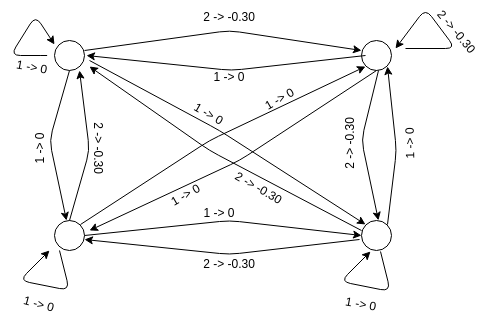
\includegraphics[width=.5\textwidth]{img/grafobase.png}
\caption{Grafo resultante de $(W)_{ij}$ y $(W')_{ij}$}
\label{fig:grafobaseconciclos}
\end{figure}

\begin{figure}[H] 
    \centering
    \begin{minipage}{0.45\textwidth}
        \centering
        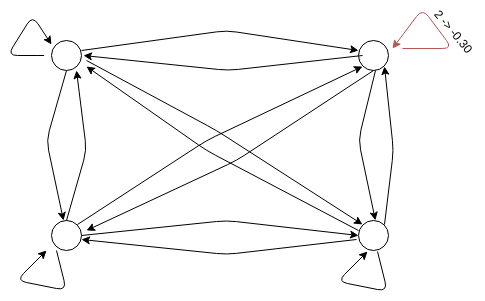
\includegraphics[width=1\textwidth]{img/ccciclosimple.png} % first figure itself
        \caption{Ciclo negativo de un solo elemento}
        \label{fig:ciclouno}
    \end{minipage}\hfill
    \begin{minipage}{0.45\textwidth}
        \centering
        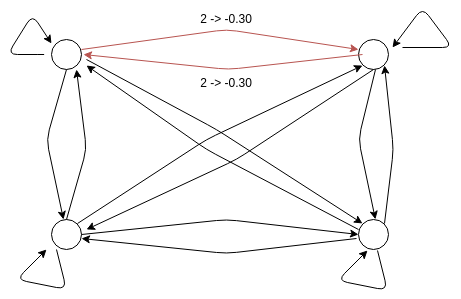
\includegraphics[width=1\textwidth]{img/ccciclodoble.png} % first figure itself
        \caption{Ciclo negativo de dos elementos}
        \label{fig:ciclodos}
    \end{minipage}\hfill
\end{figure}

\begin{figure}[H] 
    \centering
    \begin{minipage}{0.45\textwidth}
        \centering
        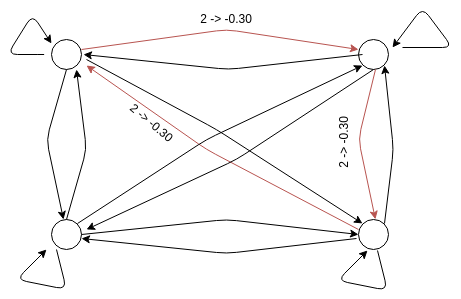
\includegraphics[width=1\textwidth]{img/ccctriple.png} % first figure itself
        \caption{Ciclo negativo de tres elementos}
        \label{fig:ciclotres}
    \end{minipage}\hfill
    \begin{minipage}{0.45\textwidth}
        \centering
        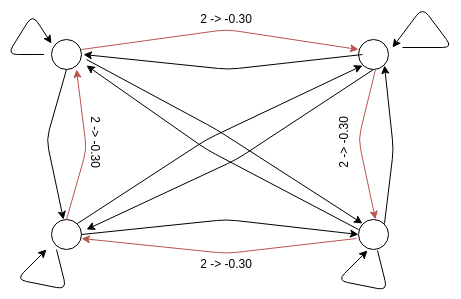
\includegraphics[width=1\textwidth]{img/ccciclocuatro.png} % first figure itself
        \caption{Ciclo negativo de cuatro elementos}
        \label{fig:ciclocuatro}
    \end{minipage}\hfill
\end{figure}

En las figuras \ref{fig:ciclouno}, \ref{fig:ciclodos}, \ref{fig:ciclotres} y \ref{fig:ciclocuatro} se obtienen un ciclos
negativos de valor $-0.3$, $-0.6$, $-0.9$ y $-1.2$ lo cual se traduce en ganacias del $100\%$, $200\%$, $300\%$ y $400\%$
de la unidad con la que se empieza. Para los alcances de este trabajo nos alcanza con que los algoritmos en cuesti\'on
devuelan cualquiera de estos ciclos.

\textbf{Ejemplo sin ciclos}\\
Sea $(W)_{ij}$ la matriz de adyacencias definida como:
    
\begin{figure}[H] 
    \centering
    \begin{minipage}{0.35\textwidth}
        \centering
\[
W=
  \begin{bmatrix}
    1 & 2 & 3 \\
    0.5 & 1 & 2 \\
    0.25 & 0.5 & 1
  \end{bmatrix}
\]
    \end{minipage}
    \begin{minipage}{0.45\textwidth}
        \centering
\[
W'=
  \begin{bmatrix}
    0 & -0.30 & 0.60 \\
    -0.30 & 0 & 0.30 \\
    -0.60 & -0.30 & 0
  \end{bmatrix}
\]
    \end{minipage}\hfill
\end{figure}


\begin{figure}[H] 
\centering
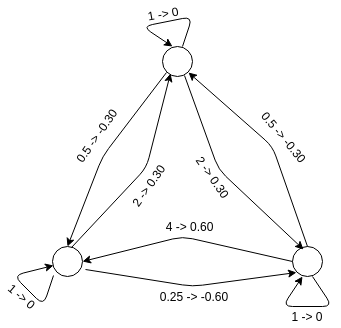
\includegraphics[width=.3\textwidth]{img/sinCiclos.png}
\caption{Grafo resultante de $(W)_{ij}$ y $(W')_{ij}$}
\label{fig:grafobaseconciclos}
\end{figure}

En este caso no existen ciclos negativos en $(W')_{ij}$ lo cual se traduce en que no existen posibilidades de arbitraje.